\documentclass[a4paper,12pt]{article}
\usepackage[T2A]{fontenc}
\usepackage[utf8x]{inputenc}
\usepackage[english,russian]{babel}
\usepackage{amsmath,amssymb,amsfonts}
\usepackage{graphicx}

\setlength{\textwidth}{16cm}
\setlength{\textheight}{25cm}
\renewcommand\baselinestretch{1.25}
\topmargin=\paperheight
\advance\topmargin-\headheight
\advance\topmargin-\headsep
\advance\topmargin-\textheight
\advance\topmargin-\footskip
\topmargin=.5\topmargin
\advance\topmargin-1truein
\oddsidemargin=\paperwidth
\advance\oddsidemargin-\textwidth
\oddsidemargin=0.5\oddsidemargin
\advance\oddsidemargin-1truein
\evensidemargin=\oddsidemargin
\tolerance1000
\emergencystretch2em


\begin{document}

\title{Разностные TVD-схемы для левой части уравнения Больцмана}
\author{Гришина В.Г, Дербакова Е.П., Колядко Г.С., Рогозин О.А.}
\date{}
\maketitle

При численном решении множества задач современной науки приходится сталкиваться с моделированием уравнения переноса \(f_t+\xi f_x=0 \).
Часто для этого применяют конечно-разностные методы.
Для адекватного описания процессов адвекции произвольных начальных условий необходимо
сочетание консервативности, монотонности и сходимости разностной схемы.
Этого легко добиться при первом порядке аппроксимации,
однако в таком случае требуются достаточно подробные разностные сетки для достижения высокой точности.
Кроме того, так называемая схемная вязкость значительным образом <<размывает>> решение со временем.
Для достижения высоких порядков аппроксимации, приходится строить нелинейные разностные схемы.
Соответствующий класс таких схем, назваемых \textit{TVD} (\textit{Total Variation Diminishing}) был впервые предложен в~\cite{Harten1983}.
Цель данной работы "--- их теоретическое и экспериментальное сравнение.

Для простоты рассмотрим одномерную прямоугольную сетку с ячейками размером \(h\),
на которой эволюционирует с временн\textit{ы}м шагом \(\tau\) разностная функция \(f_i^n = f(x_i,t_n)\).
С помощью интегро-интерполяционного метода~\cite{Samarsky1961} получается консервативная разностная схема второго порядка точности:
\[ f_i^{n+1} = f_i^n - \gamma(f_{i+1/2}^{n+1/2}-f_{i-1/2}^{n+1/2}), \]
\[ f_{i+1/2}^{n+1/2} \equiv f\left(x_i+\frac{h}{2},t_n+\frac{\tau}{2}\right)+\mathcal{O}(h^2,\tau^2)
	= f_i^n + \frac{1-\gamma}{2}\varphi(\theta_i^n)(f_{i+1}^n - f_i^n), \]
где
\[ \gamma=\frac{\xi\tau}{h}, \; \theta_i = \frac{f_i - f_{i-1}}{f_{i+1} - f_i} = 1-h\frac{f_{xx}}{f_x}+\mathcal{O}(h^2).\]
Постоянная \(\gamma\) "--- число Куранта.
Функция \(\varphi(\theta)\) называется ограничителем (англ. \textit{limiter}),
её аргумент \(\theta\) "--- показателем гладкости решения.
Схема устойчива при \(\gamma < 1\) (мы рассматриваем только положительные значения скорости,
поскольку для отрицательных формулы получаются симметричным отражением).

\begin{figure}
	\centering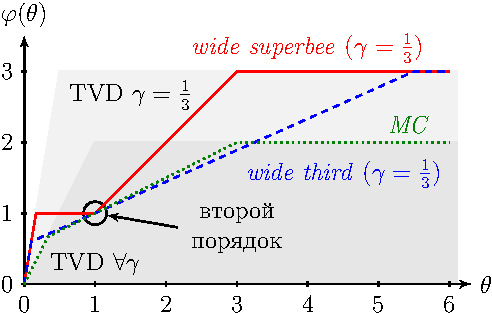
\includegraphics{sweby}
	\caption{Диаграмма Sweby}\label{fig:sweby}
\end{figure}

В работе проводится сравнение различных ограничителей, в качестве оптимальных предлагается использовать следующие два:
\[ \varphi(\theta) = \max\left(\min\left(\dfrac2{\gamma}\theta,1\right),\min\left(\theta,\dfrac2{1-\gamma}\right)\right), \]
\[ \varphi(\theta) = \min\left(\dfrac2{\gamma}\theta,\dfrac{(\gamma+1)\theta+(2-\gamma)}{3},\dfrac2{1-\gamma}\right). \]

\begin{figure}
	\centering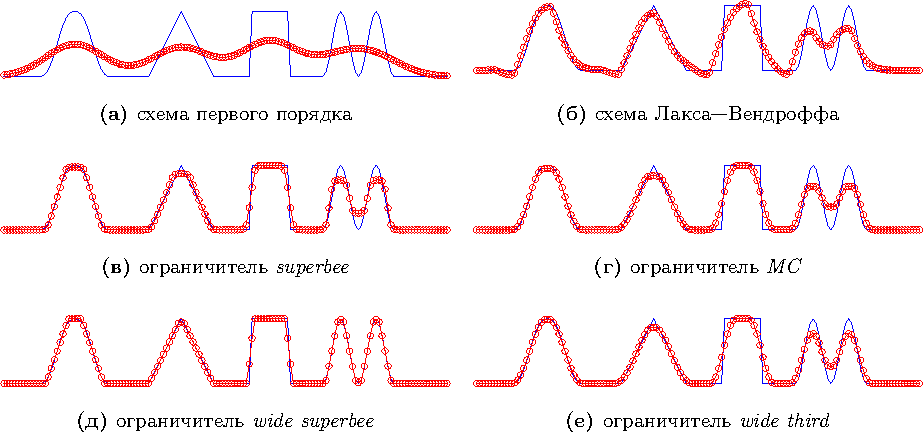
\includegraphics{limiters}
	\caption{Поведение различных схем при числе Куранта \(\gamma=1/2\) на различных начальных условиях:
		гладкое, разрыв первой производной и самой функции, наконец, при наличии быстрых осцилляций.}\label{fig:conver}
\end{figure}


Первый из них обладает максимальным порядком сходимости на разрывных решениях (единица в октаэдрической норме).
Кроме того, он рекомендуется при грубых разностных сетках и быстроосциллирующих функциях.
Он получен на основе классического ограничителя \textit{superbee}~\cite{Roe1985} с использованием расширенного (\textit{wide}) условия TVD:
\[\varphi(\theta) \leq \mathrm{minmod}\left(\frac2{\gamma}\theta,\frac2{1-\gamma}\right).\]

Второй на гладких решениях показывает максимально возможный (на пятиточечном разностном шаблоне) третий порядок сходимости,
что определяет его применимость для прецизионных вычислений.
При \(\gamma=1/2\) его центральная часть совпадает с ограничителем \textit{MC} (\textit{monotonized central-difference})~\cite{vanLeer1977}.

При решении классических задач гидрогазодинамики на основе уравнений Навье--Стокса приходится иметь дело с вектором макропараметров \(f\),
поэтому ограничитель берут независимым от \(\gamma\), однако при моделировании скалярной функции распределения
в кинетическом уравнении Больцмана, оказывается возможным использование предложенных выше улучшенных разностных схем.
Для случая \(\gamma=1/3\) они изображены на рис.~\ref{fig:sweby} в сравнении с ограничителем \textit{MC},
а на рис.~\ref{fig:conver} показаны непосредственный результат использования некоторых разностных схем.

Ограничители сраниваются как на простейшем уравнении переноса без граничных условий (похожее сравнение можно найти в \cite{Safronov2010}), 
так и на реальных задачах динимики разреженного газа.

\begin{thebibliography}{9}
\bibitem{Harten1983}
	A. Harten. High resolution schemes for hyperbolic conservation laws.
	{\it Journal of Computational Physics},
	49:~357--393, 1983.
\bibitem{Samarsky1961}
	A.A. Самарский, A.H. Тихонов. Об однородных разностных схемах.
	{\it Журнал вычислительной математики и математической физики},
	1:~5--63, 1961.
\bibitem{Roe1985}
	P.L. Roe. Some Contributions to the Modelling of Discontinuous Flows.
	{\it Large-scale computations in fluid mechanics. Lectures in Applied Mathematics},
	22:~163--193, 1985.
\bibitem{vanLeer1977}
	B. van Leer. Towards the ultimate conservative difference scheme. IV. A new approach to numerical convection.
	{\it Journal of Computational Physics},
	23(3):~276--299, 1977.
\bibitem{Safronov2010}
	A.B. Сафронов. Оценка точности и сравнительный анализ разностных схем сквозного счёта повышенного порядка.
	{\it Вычислительные методы и программирование},
	11:~137--143, 2010.

\end{thebibliography}

\end{document}
